\chapter{Software Re-engineering}

\label{Chapter3}

This section covers a simplified process of software re-engineering.
Rhat is a process for taking an existing system developing an understanding of how it works, then refactoring that system and engineering changes, then implementing the system as to the conclusions made during refactoring.

Reverse engineering is the process of reviewing the existing software systems and documenting how they function. This can be done through diagramming, documenting, and refactoring. This process allows the engineer to understand the problem domain of the system more, and also provides information on parts of the software that need to be restructured and changed.

Restructuring is the process of taking an existing design and making changes to improve the design. This is the main transitional phase that will happen after the original understanding of how the current system works through reverse engineering. Restructuring will involve reorganizing code as granular or abstract as desired. Most restructuring will focus on making small changes to the system to make it more maintainable or run more efficiently. However, the restructuring of the current system will appear to be more of an overhaul.

% Need to expand this section.
Forward engineering is the process of taking the results of the system specification created from the two previous steps of the reengineering process integrating the system into the code-base.

\section{System Understanding}

The system is arranged for the most part into different functional groups, referred to as packages. There are some exceptions to this as seen in the "ai" package, where the responsibility of controls, vision, and movement is all amalgamated together.

The flow of information is handled quite elegantly within the system.
With lower level systems passing information up to and receiving back from
higher level systems. See \ref{fig:InformationFlow} for understanding the
general idea of how this flow happens.

\begin{figure}
\centering
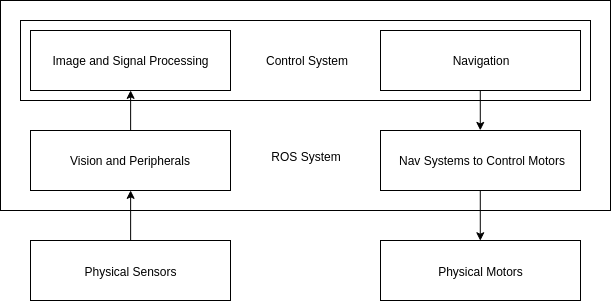
\includegraphics[width=100mm]{Figures/InformationFlow}
\decoRule
\caption[Original Information Flow]{Diagram showing how information flows in the reference frame of the control system.}
\label{fig:InformationFlow}
\end{figure}

The individual devices are handled via their own ROS nodes, which then make
the information from the devices available in a 'friendly' way.
This allows for specific driver-like programs to abstract the possibly
complex interface to the physical devices.


\section{Perceived Problems}

The control system featured no error catching or any kind of protocol to recover from an error state.
For most states the control system loops on a single state then after a condition is met will advance to the next state. This type of control system is autonomous controlling but it isn't designed for the kind of failures expected in the real world.

The control system works directly with the state information and directly handles both the condition to switch states and the assignment of the next state, see \ref{fig:DirectStateHandling}.

\begin{figure}
\centering
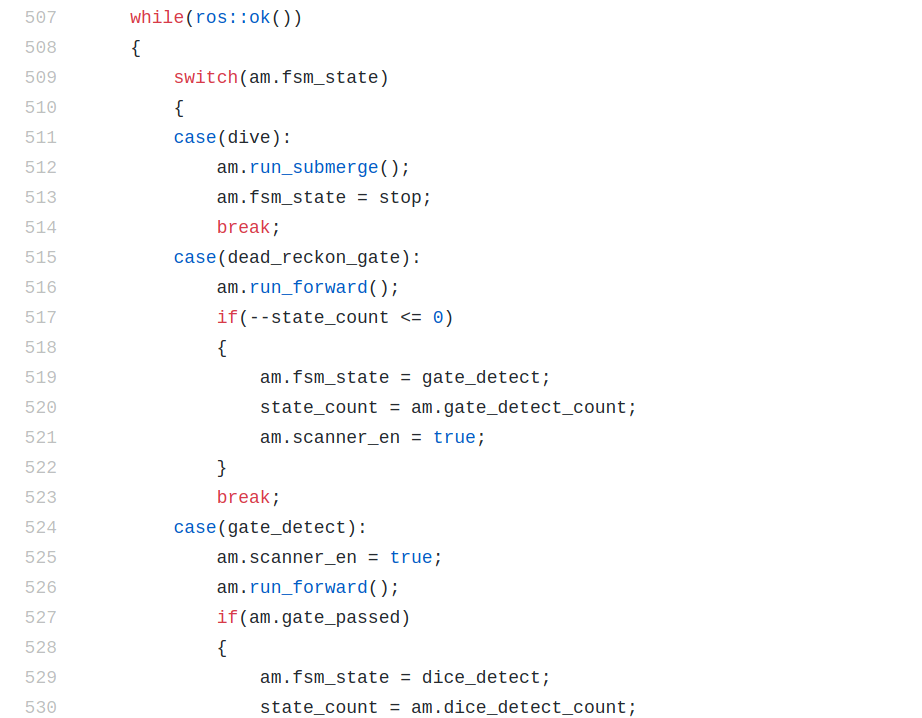
\includegraphics[width=150mm]{Figures/DirectStateHandling}
\decoRule
\caption[Direct State Handling]{Code segment showing the control systems way of handling states, controlling submarine functions, and getting information from other submarine systems.}
\label{fig:DirectStateHandling}
\end{figure}

The control system also directly handled the vision systems. The control system did offer a simple interface for the states in the state machine to utilize.


\section{Restructuring}

The control system has been assigned excessive responsibility; it performs the tasks of a control system, detection system, and navigation system. The detection systems within the control system shall be separated into a vision package and offer an interface through ROS inter process communication structures. Namely offer the same features the state machine was using, and expand the features on top of that. And the navigation system uses should also be pulled out, but an interface still be made available through ROS inter-process communication structures. To use the two new systems identified above they would need to be compatible with the existing system structure.

For the navigation system this required either using interface that existed and offered functionalities by replaced system, or a new system that acts as an interface to manage communication between old and new software systems. The latter involved much more consideration for best creating the system for usage in the future. While the former got the job done, and allowed to expand and slowly update functionality later on. Thus, the former of the two options was chosen, for the reasons given and because of time constraints for the project.

The detection systems' functionality and usage was restricted to within the control system. This allowed creation of a new system much simpler and allowed much freedom with the design of this system. Which is why the system used a simple interface to retrieve detection results, and change detection type. And this system was incorporated directly into the vision package, as having close proximity to the retrieved image files would mean for faster image processing.

The primary more generalized features to handle the support for different kinds of detection being: access to result of detection and the ability to change the current active detection algorithm which could also be set to none.

The updated version of the ROS communcation diagram was too large to embed into
this document, but it has been provided \href{https://drive.google.com/file/d/1_vJLSflxahA-7v2kYGV3wu5SfGcKEVf8/view?usp=sharing}{here}.

\begin{figure}
\centering
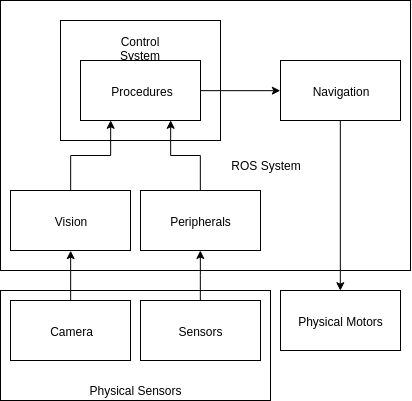
\includegraphics[width=100mm]{Figures/InformationFlowNew}
\decoRule
\caption[New Information Flow]{Diagram showing how information flows in the reference frame of the redesigned control system.}
\label{fig:InformationFlowNew}
\end{figure}

\begin{figure}
\centering
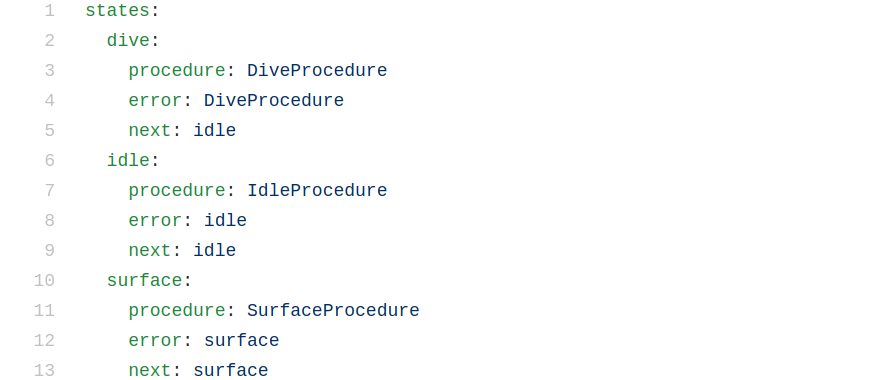
\includegraphics[width=150mm]{Figures/ExampleConfig}
\decoRule
\caption[Example Configuration File]{Shows a simple example idle configuration file. Demonstrating use of simple state organization and definition of state transitions.}
\label{fig:ExampleConfig}
\end{figure}

\section{Forward Engineering}

